\section{\textcolor{DarkBlue}{\faIcon{sliders-h}\; MDP with Increased Hazard Penalty \hfill \colorbox{orange!20}{\small 10M}}}

\begin{questionbox}
Suppose we change the MDP by penalizing the drone more for entering hazardous
states (penalty = −90). Keep γ = 0.95. [10M] \\
(a) What are the resulting optimal value function and policy? Explain the difference
(if any) in the solution due to changing the problem in the two MDPs. Focus on
the regions near hazardous cells. [3M] \\
(b) Is there are scenario where hovering may be preferred? Explain either ways. [2M] \\
(c) Is there are scenario when a longer path to the fire zone is preferable from a
particular cell? Why or why not? [2M] \\
(d) Given the above MDP with the −90 hazard penalty and γ = 0.95, suppose the
wind becomes stronger. As a result, in all non-terminal states, the drone moves
in the intended direction with a chance of 40%, in either of the perpendicular
direction with a chance of 25%, and stays in same the cell rest of the times.
Comment your thoughts on the solution to the resulting MDP. [3M]
\end{questionbox}

\begin{solutionbox}

\subsection*{\textcolor{Cerulean}{(a) Optimal Value Function \& Policy with $-90$ Hazard Penalty}}

With $-90$ smoke penalty and $\gamma=0.9$, smoke regions become \emph{negative convergence zones}.

\begin{figure}[H]
\centering
\begin{minipage}{0.42\textwidth}
    \centering
    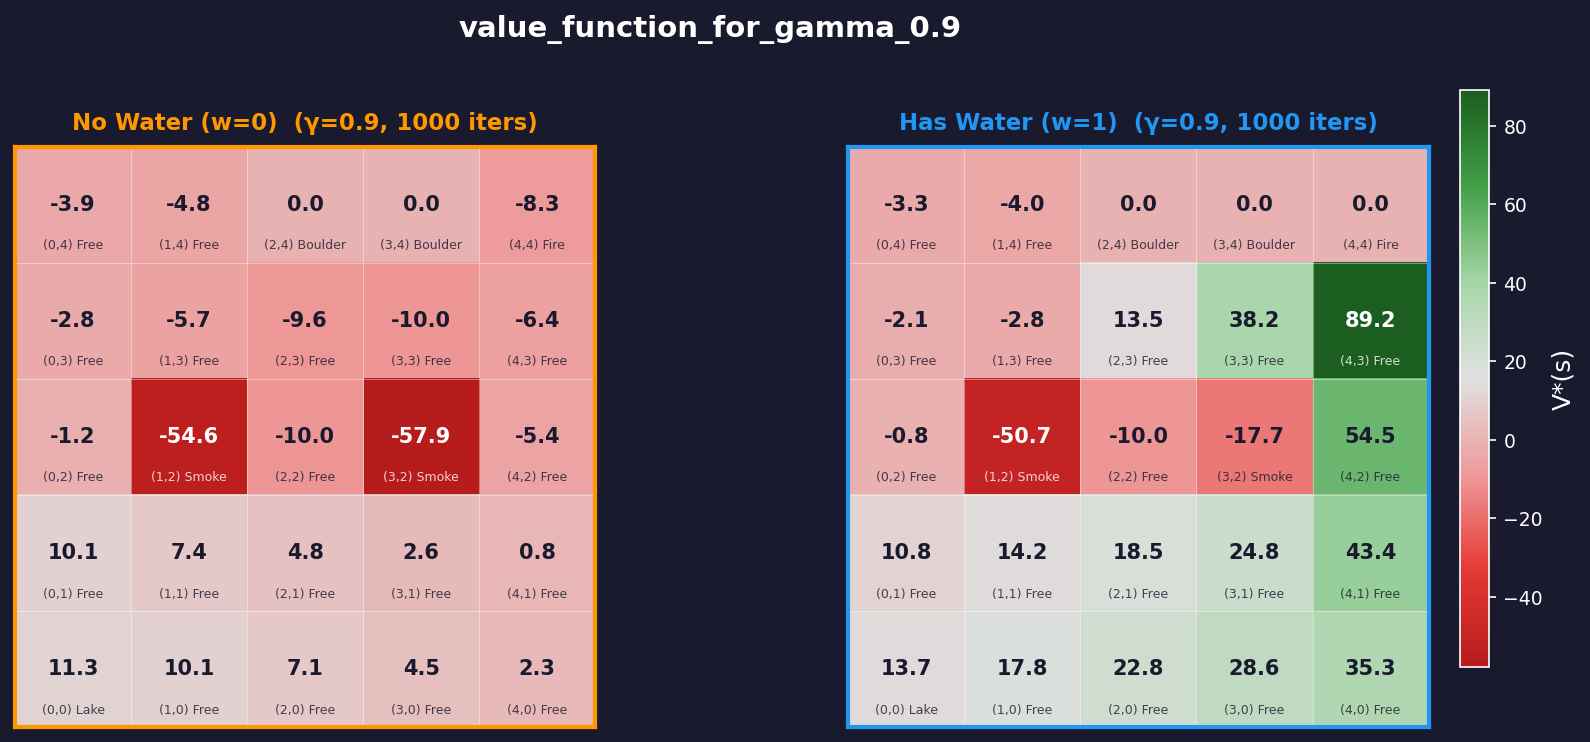
\includegraphics[width=\textwidth]{images/value_function_for_gamma_0.9.png}
\end{minipage}
\hfill
\begin{minipage}{0.42\textwidth}
    \centering
    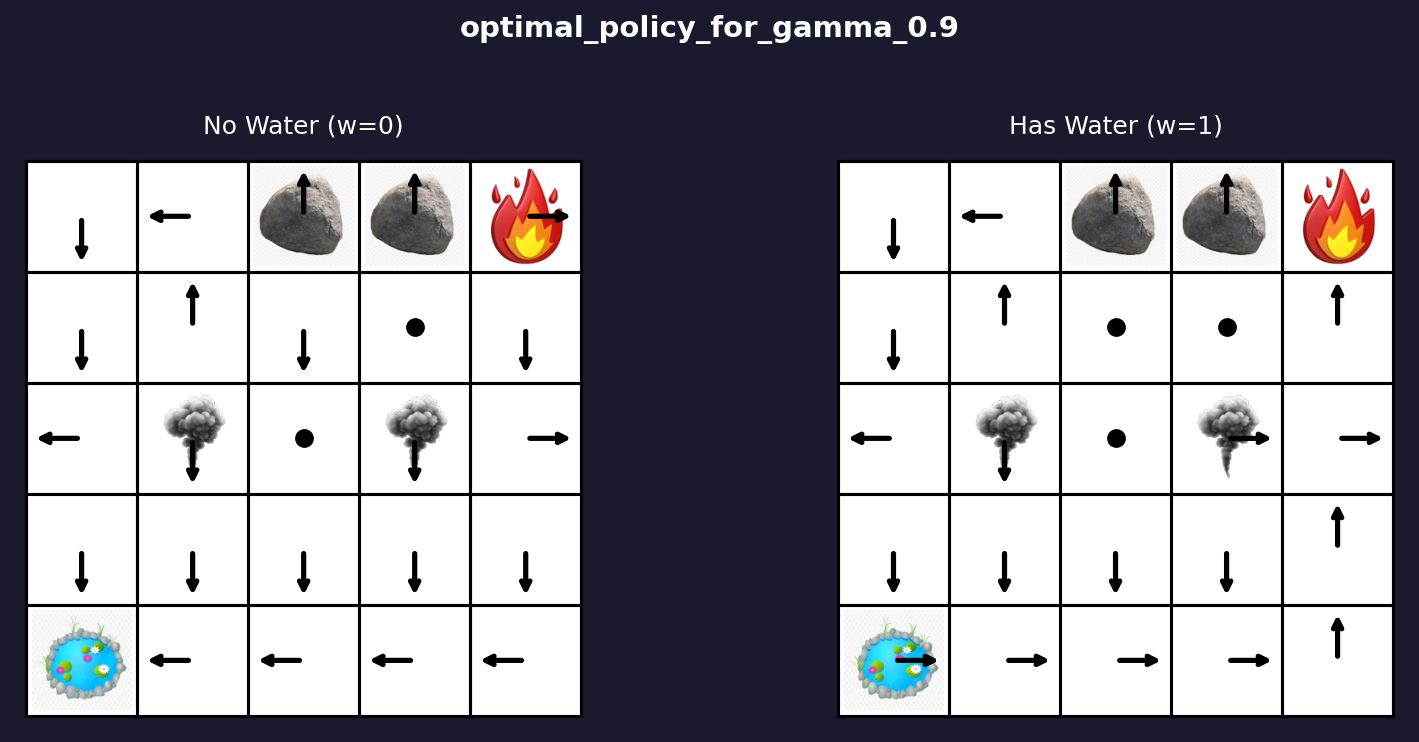
\includegraphics[width=\textwidth]{images/optimal_policy_for_gamma_0.9.png}
\end{minipage}
\captionof{figure}{Value function and policy ($\gamma=0.9$, hazard $=-90$).}
\end{figure}

\vspace{-0.8em}

\textbf{Key observations:} (i) Smoke nearly as bad as boulders; (ii) $(4,2)$ avoids despite 2-step proximity due to drift; (iii) Slower convergence—balanced immediate/future penalties; (iv) Planning: $\gamma=0.3\to1.4$ steps, $0.9\to10$, $0.95\to20$.

\subsection*{\textcolor{Cerulean}{(b) Hovering Scenarios}}

\textbf{Yes}, surprisingly $\gamma=0.9$ has \textbf{5/50 hovering states} (most of all): $(3,3)$ and $(4,3)$ with $w\in\{0,1\}$; $(1,3)$ with $w=0$.

\textbf{``Indecision Threshold'':} At $\gamma=0.3$, shortsighted—best action obvious (minimal hovering). At $\gamma=0.95$, farsighted—clear long-term strategy (minimal hovering). At $\gamma=0.9$, immediate/future rewards have \emph{equal weight}, creating ambiguity. Q-values for competing actions nearly identical; Bellman updates ``waver.'' Result: maximum hovering. Paradox: more hovering than myopic $\gamma=0.3$ because caught between timescales, not from shortsightedness.

\subsection*{\textcolor{Cerulean}{(c) Longer Path Preference}}

\textbf{Yes.} Example: from smoke $(1,2)$, the optimal policy takes a long detour (see Fig.) rather than the direct 3-step path to fire $(4,4)$.

\begin{figure}[H]
\centering
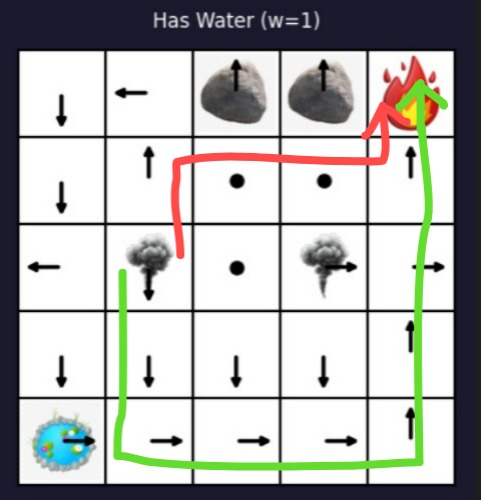
\includegraphics[width=0.35\textwidth]{images/prefered_long_path.jpeg}
\captionof{figure}{Long detour from $(1,2)$ to avoid hazards.}
\end{figure}

\vspace{-0.8em}

\textbf{Reason:} The short path passes through 2 boulders $\{(2,4),(3,4)\}$ and smoke $(3,2)$. With stochastic wind, cumulative hazard-hit probability is too high. The long path—even using off-grid bouncebacks—minimizes $-90$ smoke and $-100$ boulder risks. When hazard penalties are severe, safety beats efficiency.

\subsection*{\textcolor{Cerulean}{(d) Stronger Wind Analysis}}

Stronger wind ($P_{\text{fwd}}=0.4$, $P_{\text{perp}}=0.25$ each, $P_{\text{stay}}=0.1$) degrades control significantly:

\begin{figure}[H]
\centering
\begin{minipage}{0.42\textwidth}
    \centering
    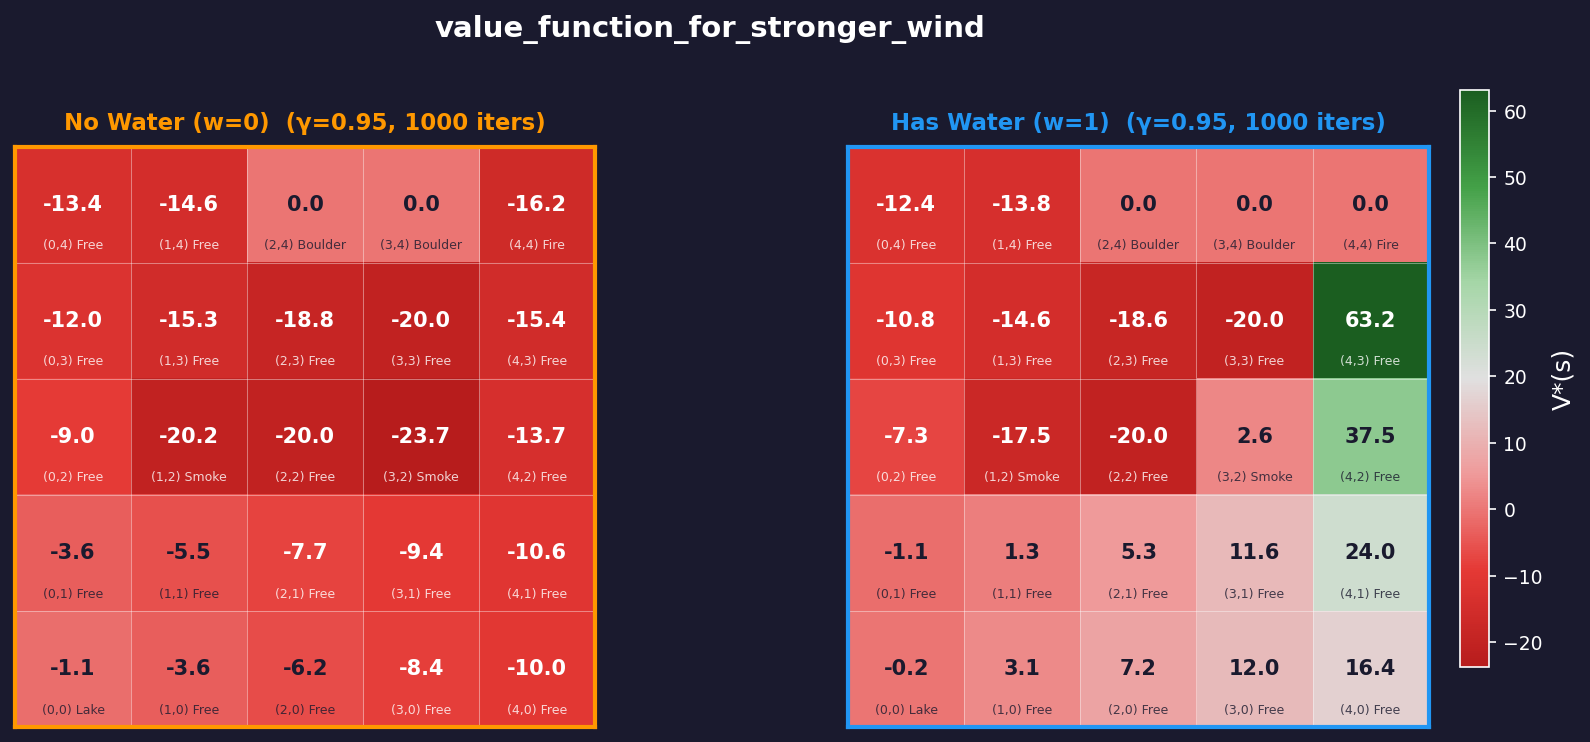
\includegraphics[width=\textwidth]{images/value_function_for_stronger_wind.png}
\end{minipage}
\hfill
\begin{minipage}{0.42\textwidth}
    \centering
    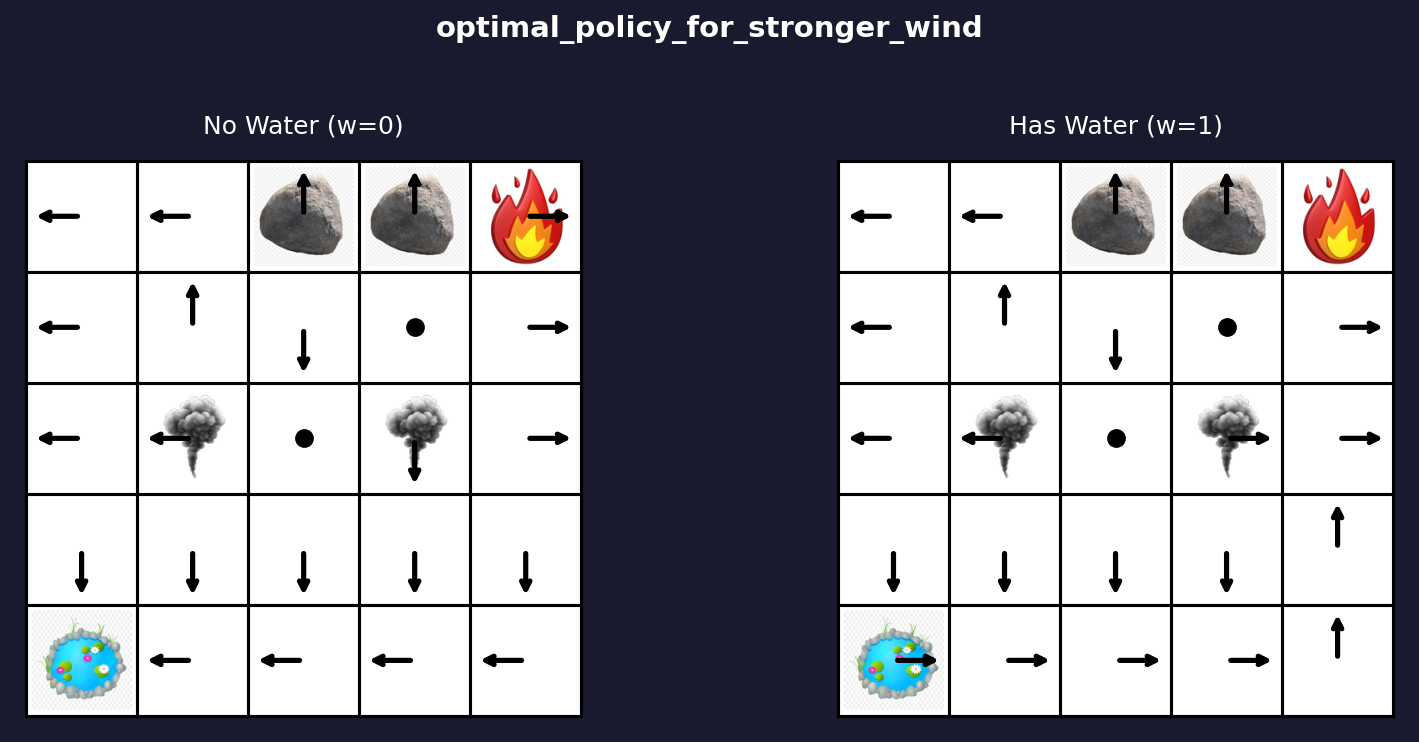
\includegraphics[width=\textwidth]{images/optimal_policy_for_stronger_wind.png}
\end{minipage}
\captionof{figure}{Value function and policy with stronger wind ($\gamma=0.95$, hazard $=-90$).}
\end{figure}

\vspace{-0.8em}
\textbf{Key observations:}
\textbf{1. Increased stochasticity:} Perpendicular drift rises from 10\% to 25\% (2.5× higher)—movement becomes much less predictable.
\textbf{2. Control degradation:} Forward probability drops from 70\% to 40\% (↓43\%); total perpendicular risk rises from 20\% to 50\% (↑150\%). Result: \emph{half} of all movements now go sideways.
\textbf{3. Lower value functions:} Expected cumulative rewards decrease across all states due to higher chance of unintended hazard encounters.
\textbf{4. More conservative policy:} Agent prefers wider safety margins around hazards, more hovering in ambiguous locations, longer detour paths to avoid risk corridors.
\textbf{5. Convergence behavior:} Took more iterations due to increased uncertainty in Bellman updates.
Combined with $-90$ smoke penalties, this creates ``no-go zones'' where smoke regions become near-impassable. Models storm degradation scenarios where control authority severely compromised.
\end{solutionbox}